\documentclass{article}
\usepackage[UTF8]{ctex}
\usepackage{geometry}
\geometry{a4paper,left=1cm,right=1cm,top=1cm,bottom=2cm}
\usepackage{amsmath}
\usepackage{booktabs}
\usepackage{amsfonts}
\usepackage{graphicx}
\usepackage{float}
\usepackage[utf8]{inputenc}
\usepackage[T1]{fontenc}
\usepackage{tcolorbox}
\usepackage[colorlinks,linkcolor=blue]{hyperref}

\begin{document}
\title{\textbf{从NCE到InfoNCE}}
\maketitle
\centerline{\author{Huacheng Li}}
\begin{abstract}
    NCE的作用就是
\end{abstract}

\begin{table}[H]
    \caption{符号总结}
    \label{TAB:GlobalSymble}
    \centering
    \begin{tabular}{p{4cm} p{10cm}}
        \toprule
        \textbf{Symbol}       & \textbf{Definations}  \\ 
        \midrule
        $\mathcal{V}=\{v_1, v_2, \ldots, v_{|\mathcal{V}|}\}$ & 词汇表\\
        $\mathcal{S}=\{s_1, s_2, \ldots, s_{|\mathcal{S}|}\}$ & 语料库,即所有的句子\\
        $s=\{w_1, w_2, \ldots, w_m\}$ & 一条语句,其组成单元是单词 \\
        $c_i$ & 句子$s$中单词$w_i$的上下文\\
        $p(w_i|c_i)$ & 以$c_i$为上下文,下一个单词为$w_i$的概率,这也是真正的语言模型 \\
        $p_\theta(w|c)$ & 表示我们建立的以$\theta$为参数的语言模型,之所以去掉$i$,是因为要表示所有单词的概率 \\
        $p_{data}(w|c)$ & 表示从data中采样得到的概率分布\\
        $p_{noise}(w)$ & 表示从噪声分布中采样得到的概率分布\\
        $p_{sample}(w|c)$ & 表示$p_{data}$与$p_{noise}$的混合分布,因为都是采样得到的。\\
        $s_\theta(w,c)$ & 神经网络输出的单词$w$与上下文$c$的匹配程度,注意这里没有表示为条件概率 \\
        $u_\theta(w,c) = \exp (s_\theta (w,c))$ & Softmax处理匹配度的分子\\
        \bottomrule
    \end{tabular}
  \end{table} 




\section{从NLP视角引入NCE}
\label{sec:NLP}
\subsection{n-gram}
\label{sec:NLP:NGRAM}
假定单词库表示为$\mathcal{V} = \{v_1, v_2, \ldots, v_{|\mathcal{V}|}\}$。
语料库$\mathcal{S} = \{s_1, s_2, \ldots, s_{|\mathcal{S}|}\}$是语句的集合。
语言模型假设所有可能的句子服从一个概率分布,每个句子出现的概率之和为1。
合理的句子出现的概率高,不合理的句子出现概率低。
句子$s=\{w_1, w_2, \ldots, w_m\}$,其出现的概率可以表示为公式 (\ref{EQ:ALLGRAM}), 其中$c_i$表示单词$w_i$的上下文。
\begin{equation}
    \begin{split}
        p(s)=p(w_1,w_2,\ldots,w_m)&=p(w_1)*p(w_2|w_1)*p(w_3|w_1,w_2)*\cdots*p(w_m|w_1,\ldots,w_{m-1})\\
        &=\prod_{i=1}^{m} p(w_i|w_1,\ldots,w_{i-1})\\
        &=\prod_{i=1}^{m} p(w_i|c_i)
    \end{split}
    \label{EQ:ALLGRAM}
\end{equation}

n-gram假设一个词的上下文只与前n个词有关,因此n-gram可以将模型进化为公式(\ref{EQ:NGRAM})
\begin{equation}
    p(w_1,w_2,\ldots,w_m)=\prod_{i=1}^{m} p(w_i|w_{i-n+1},\ldots,w_{i-1})
    \label{EQ:NGRAM}
\end{equation}

\subsection{最大似然估计}
\label{sec:NLP:MLE}
n-gram模型建立之后,根据语料库中$w_i$和$c_i$,计算$p(w_i|c_i)$。
\textit{在计算一个句子出现的概率时,将这个句子中出现的$p(w_i|c_i)$连乘。}
因此,可以不计算每个$w$和$c$的概率,而是建立一个目标函数,根据语料库去求解这些概率。
可以将$w$和$c$的关系看成一个依赖参数$\theta$的条件分布$p_\theta (w_i|c_i)$。
因此优化目标可以如下所示
\begin{equation}
    \mathcal{L}_{MLE}=\sum_{w_i\in s}\log p_\theta (w_i|c_i)
    \label{EQ:NGRAM_MLE}
\end{equation}
条件概率$p_\theta (w_i|c_i)$可以看作参数为$\theta$的函数$F(w,c;\theta)$。
通过最优化参数$\theta^*$得到函数$F$。


\subsection{神经概率语言模型}
\label{sec:NLP:NPLM}

上述方法问题主要在于两点:
\begin{itemize}
    \item 如何构造函数$F$
    \item 最大似然估计理论可行,但计算量太大
\end{itemize}

针对第一个问题,引入神经网络来拟合函数$F$,\cite{DBLP:journals/jmlr/BengioDVJ03}等人提出NPLM (Neural Probabilistic Language Model),不再受限与gram的大小,可以包含任意大小上下文的情况建模词的条件概率$p(w|c)$。
假设单词库$\mathcal{V} = \{v_1, v_2, \ldots, v_{|\mathcal{V}|}\}$。将$(w,c)$看作训练样本,通过神经网络和softmax后会输出一个向量$\hat{y}_i=\{\hat{y}_{i,1}\}$。
每一维$\hat{y}_{i,j}=p(v_j|c_i)$表示当上下文为$c_i$时,对应的第$i$个位置的单词$w_i$是单词库中第$j$个单词$v_j$的概率。
训练过程要求最后单词库中概率最大的单词就是训练样本中对应的单词$w_i$。
因此,\textbf{NPLM将语言模型的建立看作是多分类问题}。

\begin{tcolorbox}[title = NPLM解释]
假定单词库是$V = \{v_1, v_2, \ldots, v_{|V|}\}$。任意一个句子$s = \{w_1, w_2, \ldots, w_m\}$,假定可见序列为$c_l = (w_1, w_2,\ldots, w_{l-1})$,我们希望根据$c_l$预测下一个单词$w_l$。
也就是建模概率$p(w|c)$,NPLM选择使用神经网络来拟合这个概率分布,也就是$p(w|c)=F_{\theta}(w,c)$。也就是能够对于任意上下文$c$,神经网络能够计算每一单词对应的概率,也可以理解为能够针对一组输入$(w,c)$,输出它对应的概率。

在这个场景下,$w \in \mathcal{R}^d$,$c \in \mathcal{R}^d$,$y\in F_\theta(w,c) \in \mathcal{R}^{|V|}$。通常意义上讲,最后一步输出$y$要经过Softmax处理,输出的logits转换为归一化的概率。

这里要尤其注意的是,由于神经网络的输入和处理的都是向量,向量中值的分布对应着语义。\textbf{\textcolor{red}{神经网络能够对语义建模,本质上还是能够对这种向量的值的分布进行建模,也就是让神经网络学习语义的分布。}}

\end{tcolorbox}

假定输入softmax之前的结果用$s_\theta(w,c)$表示【个人理解,也就是神经网络输出的logits,即单词$w$和上下文$c$在参数为$\theta$的语言模型下的匹配程度,即未归一化的概率】,那么$w$的条件概率可以表示为:
\begin{equation}
    p_\theta(w|c)=\frac{e^{s_\theta(w,c)}}{\sum_{w^{'}\in V}e^{s_\theta(w^{'},c)}} = \frac{u_\theta(w,c)}{Z(c)}
    \label{EQ:NPLM_SOFTMAX}
\end{equation}
其中,$u_\theta(w,c)=e^{s_\theta(w,c)}$表示下一个单词是这个单词$w$的概率,$Z(c)=\sum_{w^{'}\in V}e^{s_\theta(w^{'},c)}$表示当前单词库中所有单词的概率累计,也叫配分函数或归一化因子。
\textbf{由于单词库规模很大,配分函数难以计算,因此引入NCE}。

将公式(\ref{EQ:NPLM_SOFTMAX})看作函数$F$的具体形式,使用章节\ref{sec:NLP:MLE}提到的最大似然估计求解参数$\theta$。
\textbf{我们只能够根据训练数据优化模型,得到最佳参数$\theta^{*}$。即我们希望在最佳参数$\theta^{*}$对应的模型能够最好地拟合训练数据。也就是训练数据的MLE最大。将从句子$c$中取样的关于$w$的分布看作经验分布$p_{data}(w|c)$},可以将公式(\ref{EQ:NGRAM_MLE})重写为下式:
\begin{equation}
    \mathcal{L}_{MLE} = \sum_{w \sim p_{data}(w|c)} \log p_\theta (w|c) = \mathbb{E}_{w \sim p_{data}(w|c)} \log \frac{u_\theta(w,c)}{Z(c)}
    \label{EQ:NPLM_MLE_EMPRICAL}
\end{equation}
最大化经验分布即是对$\theta$求导:
\begin{equation}
    \begin{split}
        \frac{\partial}{\partial \theta} \mathcal{L}_{MLE} &= \mathbb{E}_{w \sim p_{data}(w|c)} \frac{\partial}{\partial \theta} \log \frac{u_\theta (w,c)}{Z(c)} \\
        &= \mathbb{E}_{w \sim p_{data}(w|c)} [ \frac{\partial}{\partial \theta} \log u_\theta (w,c) - \frac{\partial}{\partial \theta} \log Z(c)] \\
        &= \mathbb{E}_{w \sim p_{data}(w|c)} \frac{\partial}{\partial \theta} \log u_\theta (w,c) - \frac{\partial}{\partial \theta} \log Z(c)
    \end{split}
    \label{EQ:Derive_MLE}
\end{equation}
上式最后一步中,$Z(c)=\sum_{w^{'}\in V}e^{s_\theta(w^{'},c)}$表示当前单词库中所有单词的概率累计,$w^{'}$为单词库中所有的单词,每个单词的概率由$p_\theta(w|c)$产生。
\textbf{尽管$w^{'}\sim p_\theta(w|c)$与参数$\theta$有关,但与经验分布$w \sim p_{data}(w|c)$无关,因此需要对后一项求导,但可以把期望去掉}。
对$Z(c)$求导如下:
\begin{equation}
    \begin{split}
        \frac{\partial}{\partial \theta} \log Z(c) &= \frac{1}{Z(c)} \frac{\partial}{\partial \theta}Z(c) \\
        &= \frac{1}{Z(c)} \frac{\partial}{\partial \theta} \sum_{w^{'}\in V} u_\theta(w^{'},c) \\
        &= \frac{1}{Z(c)} \frac{\partial}{\partial \theta} \sum_{w^{'}\in V} \exp(u_\theta(w^{'},c)) \\
        &= \sum_{w^{'} \in V} \frac{1}{Z(c)} \exp(s_\theta(w^{'},c)) \frac{\partial}{\partial \theta}s_\theta(w^{'},c) \\
        &= \sum_{w^{'}\in V} p_\theta (w^{'}, c) \frac{\partial}{\partial \theta}s_\theta(w^{'},c)\\
        &= \mathbb{E}_{w \sim p_\theta (w|c)}\frac{\partial}{\partial \theta} s_\theta (w,c) //\textbf{因为这里$w$和$w^{'}$没有区别} \\
        &= \mathbb{E}_{w \sim p_\theta (w|c)}\frac{\partial}{\partial \theta} \log u_\theta (w,c) //\textbf{这个和上一个等价,一个是指数,一个是对数} \\
    \end{split}
    \label{EQ:Derive_Z}
\end{equation}
将公式(\ref{EQ:Derive_Z})代回公式(\ref{EQ:Derive_MLE}),可以得到下式:
\begin{equation}
    \begin{split}
        \frac{\partial}{\partial \theta} \mathcal{L}_{MLE} &= \mathbb{E}_{w \sim p_{data}(w|c)} \frac{\partial}{\partial \theta} \log u_\theta(w,c) - \frac{\partial}{\partial \theta} \log Z(c) \\
        &= \mathbb{E}_{w \sim p_{data}(w|c)} \frac{\partial}{\partial \theta} \log u_\theta(w,c) - \mathbb{E}_{w \sim p_\theta(w|c)} \frac{\partial}{\partial \theta} \log u_\theta(w,c)\\
        &= \sum_{w} p_{data}(w|c) \frac{\partial}{\partial \theta} \log u_\theta (w,c) - \sum_{w} p_\theta (w,c)\frac{\partial}{\partial \theta} \log u_\theta (w,c) \\
        &= \sum_{w}[(p_{data}(w|c)-p_\theta(w|c))\frac{\partial}{\partial \theta} \log u_\theta (w,c)]
    \end{split}
    \label{EQ:NPLM_MLE_DERIVE}
\end{equation}
如上式所示,最终还是绕不开归一化常数$Z(c)$

\section{什么是NCE}
\label{sec:NCE}
为解决上一章中$Z(c)$计算复杂的问题,有以下几种思路:
\begin{itemize}
    \item 将$Z(c)$看作一个参数训练:\textbf{不可行},因为由公式(\ref{EQ:NPLM_MLE_EMPRICAL})可以看出,训练过程有可能会直接让$Z(c)$趋向于0
    \item 不定义$Z(c)$,直接使用$u_\theta(w,c)$估计模型:不在文本讨论范围,如 Contrastive Divergence \cite{DBLP:journals/neco/Hinton02},Score Matching \cite{DBLP:journals/jmlr/Hyvarinen05}。
    \item NCE:\emph{核心思想就是通过学习数据分布样本和噪声分布样本之间的差别,从而发现数据中的特性}。通过最大化同一个目标函数来估计模型参数$\theta$和归一化常数。\emph{NCE将Z(c)推断问题转化为二分类问题,训练分类器能够对数据样本和噪声样本进行二分类,这样分类器的参数$\theta$等价于我们要学习的参数$\theta$}。也可以说是,我们想要建立一个参数为$\theta$的语言模型,对上下文$c$,对目标单词$w$的预测概率$p_{\theta}(w|c)$尽可能接近数据集中分布$p_{data}(w|c)$。
\end{itemize}

\subsection{从数据集中采样概率}

假设特定上下文$c$的数据分布为$p_{data}(w|c)$,我们称从它里面取出的样本为\textbf{正样本},令其为类别$D=1$;与上下文无关的噪声分布为$p_{noise}(w)$,即随机采的,取出的为\textbf{负样本},类别为$D=0$。
如果取出的正样本数和负样本数分别为$k_d$和$k_n$。正负样本混合得到混合分布$p_{sample}(w|c)$。

\begin{equation}
    \begin{cases}
        p_{sample}(D=1|w,c)=\frac{k_d}{k_d+k_n}\\
        p_{sample}(D=0|w,c)=\frac{k_n}{k_d+k_n}\\
        p_{sample}(w|D=1,c)=p_{data}(w|c) \\
        //\text{上式可以理解为,已知取正例,且从上下文$c$相关空间取样的概率}\\
        p_{sample}(w|D=0,c)=p_{noise}(w)
    \end{cases}
\end{equation}

所以后验概率可以计算为
\begin{equation}
    \begin{split}
        p_{sample}(D=0|w,c)&=\frac{p_{sample}(D=0,w|c)}{p(w|c)}\\
        &= \frac{p_{sample}(D=0)p_{sample}(w|D=0,c)}{p_{sample}(D=0)p_{sample}(w|D=0,c)+p_{sample}(D=1)p_{sample}(w|D=1,c)}\\
        &= \frac{\frac{k_n}{k_n+k_d} \times p_{noise}(w)}{\frac{k_d}{k_d+k_n} \times p_{data}(w|c) + \frac{k_n}{k_n+k_d} \times p_{noise}(w)} \\
        &= \frac{\frac{k_n}{k_d} \times p_{noise}(w)}{p_{data}(w|c)+\frac{k_n}{n_d} \times p_{noise}(w)}
    \end{split}
\end{equation}


\begin{equation}
    \begin{split}
        p_{sample}(D=1|w,c)&=\frac{p_{sample}(D=1,w|c)}{p_{sample}(w|c)}\\
        &= \frac{p_{sample}(D=1) p_{sample}(w|D=1,c)}{p_{sample}(D=0)p(w|D=0,c) + p_{sample}(D=1)p_{sample}(w|D=1,c)}\\
        &= \frac{\frac{k_d}{k_d+k_n}\times p_{data}(w|c)}{\frac{k_d}{k_d+k_n} \times p_{data}(w|c) + \frac{k_n}{k_n+k_d} \times p_{noise}(w)}\\
        &= \frac{p_{data}(w|c)}{p_{data}(w|c)+\frac{k_n}{n_d} \times p_{noise}(w)}
    \end{split}
\end{equation}

令负样本和正样本数目的比例为$k=\frac{k_n}{k_d}$:
\begin{equation}
    \begin{cases}
        p_{sample}(D=0|w,c)=\frac{k \times p_{noise}(w)}{p_{data}(w|c) + k \times p_{noise}(w)}\\
        p_{sample}(D=1|w,c)=\frac{p_{data}(w|c)}{p_{data}(w|c) + k \times p_{noise}(w)}
    \end{cases}
    \label{EQ:NCE_Simplification}
\end{equation}

\subsection{如何用采样近似语言模型}

我们的训练目标是将似然函数在整个数据集上的期望最大化,即下式的最大化
\begin{equation}
    \mathbb{E}_{w \sim p_{sample}(w|c)} \left[\log p_\theta(d|w,c) \right]
\end{equation}
下面要解释该公式的含义。其中符号含义如下所示:
\begin{itemize}
    \item $d$表示数据集,所有的$w$都是从$d$中采集的。
    \item $p_{data}(w|c)$表示从真实数据集中采样的真实数据样本的概率
    \item $p_{noise}(w)$表示噪声分布采集的,以语境$c$为条件下的样本分布
    \item $p_{sample}(w|c)$表示混合分布中,语境$c$为条件下单词$w$的概率。
\end{itemize}
由于我们无法知道真正的数据分布$p_{data}(w|c)$。只能通过$p_{\theta}(w,c)$来近似。即使$p_{\theta}(w|c)$,即通过在在数据中采样的结果计算loss,更新参数$\theta$,逐步使函数$p_{\theta}(w|c)$逼近$p_{data}(w|c)$。因此,我们希望语言模型$p_{\theta}(w|c)$的预测结果能够尽可能的与真实数据相似。也就是如下期望的最大化。

\begin{equation}
    \mathbb{E}_{w \sim p_{sample}(w|c)} \left[\log p_\theta(d|w,c) \right]
\end{equation}

由于上文提到,噪声的强度(样本数量)是真实样本的$k$倍,我们可以将混合分布表示为

\begin{equation}
    p_{sample}(w|c) = \frac{1}{1+k}p_{data}(w|c) + \frac{k}{1+k} p_{noise}(w) = \frac{p_{data}(w|c)+ k \cdot p_{noise}(w)}{1+k}
\end{equation}

,因此上式可以展开为
\begin{equation}
    \begin{split}
        \mathbb{E}_{w \sim p_{sample}(w|c)} \left[\log p_\theta (d|w,c)\right] &= \int_{w} p_{sample}(w|c) \log p_{\theta}(d|w,c)dw \\
        &= \int_w \frac{p_{data}(w|c)+ k \cdot p_{noise}(w)}{1+k} \cdot \log p_{\theta}(w|c) dw \\
        &= \frac{1}{1+k} \int_w \left[p_{data}(w|c) + k \cdot p_{noise}(w|c)\right] \log p_{\theta} (d|w,c) dw \\
        &= \frac{1}{1+k} \left[ \int_w p_{data}(w|c) \log p_{\theta}(d|w,c) dw + k \int_w p_{noise}(w) \log p_\theta(d|w,c) dw \right] \\
        &= \frac{1}{1+k} \{ \mathbb{E}_{w \sim p_{data}(w|c)} \left[ \log p_{\theta}(d|w,c) \right]  + k  \mathbb{E}_{w \sim p_{noise}(w)} \left[ \log p_{\theta}(d|w,c)  \right]\}\\
        &= \frac{1}{1+k} \{ \mathbb{E}_{w \sim p_{data}(w|c)} \left[ \log p_{\theta}(D=1|w,c) \right]  + k  \mathbb{E}_{w \sim p_{noise}(w)} \left[ \log p_{\theta}(D=0|w,c)  \right]\}\\
        &= \frac{1}{1+k} \{ \mathbb{E}_{w \sim p_{data}(w|c)} \left[ \log \frac{p_\theta(w|c)}{p_\theta(w|c)+k \cdot p_{noise}(w)} \right] \\ &+ k  \mathbb{E}_{w \sim p_{noise}(w)} \left[ \log \frac{k \cdot p_{noise}(w)}{p_\theta(w|c)+k \cdot p_{noise}(w)}  \right]\}\\
    \end{split}
\end{equation}

对于语境$c$,我们可以将其目标函数写为:
\begin{equation}
    \mathcal{J}^c(\theta) = \mathbb{E}_{w \sim p_{data}(w|c)} \left[ \log \frac{p_\theta(w|c)}{p_\theta(w|c)+k \cdot p_{noise}(w)} \right]  + k  \mathbb{E}_{w \sim p_{noise}(w)} \left[ \log \frac{k \cdot p_{noise}(w)}{p_\theta(w|c)+k \cdot p_{noise}(w)}  \right] 
\end{equation}
然后我们计算关于$\theta$的导数:
\begin{equation}
    \begin{split}
        \frac{\partial}{\partial \theta} \mathcal{J}^c (\theta)  &= \frac{\partial}{\partial \theta} \mathbb{E}_{w \sim p_{data}(w|c)} \left[ \log \frac{p_\theta(w|c)}{p_\theta(w|c)+k \cdot p_{noise}(w)} \right]  + k \frac{\partial}{\partial \theta}  \mathbb{E}_{w \sim p_{noise}(w)} \left[ \log \frac{k \cdot p_{noise}(w)}{p_\theta(w|c)+k \cdot p_{noise}(w)}  \right] \\
        &= \begin{matrix}
            \underbrace{\mathbb{E}_{w \sim p_{data}(w|c)} \left[ \frac{\partial}{\partial \theta} \log \frac{p_\theta(w|c)}{p_\theta(w|c)+k \cdot p_{noise}(w)} \right]} & + & \underbrace{k  \mathbb{E}_{w \sim p_{noise}(w)} \left[ \frac{\partial}{\partial \theta} \log \frac{k \cdot p_{noise}(w)}{p_\theta(w|c)+k \cdot p_{noise}(w)}  \right]} \\
            <1> & & <2> \\
        \end{matrix}
    \end{split}
\end{equation}

接下来分别对$<1>$和$<2>$中括号部分求解展开。对于<1>式,可以重写为:

\begin{equation}
    \begin{split}
        \frac{\partial}{\partial \theta} \log \frac{p_\theta(w|c)}{p_\theta(w|c)+k \cdot p_{noise}(w)} &= \frac{\partial}{\partial \theta} (- \log \frac{p_\theta(w|c)+k \cdot p_{noise}(w)}{p_\theta(w|c)}) = \frac{\partial}{\partial \theta} \left[ -\log(1+ \frac{k \cdot p_{noise}(w)}{p_{\theta}(w|c)}) \right] \\
        &= - \frac{1}{1 + \frac{k \cdot p_{noise}(w)}{p_\theta (w|c)}} \{ 0 + \frac{- k \cdot p_{noise}(w)}{\left[ p_\theta(w|c) \right]^2} \frac{\partial}{\partial \theta} p_\theta(w|c) \}\\
        &= \frac{p_\theta(w|c)}{p_\theta(w|c) + k \cdot p_{noise}(w)} \frac{ k \cdot p_{noise}(w)}{\left[ p_\theta(w|c) \right]^2} \frac{\partial}{\partial \theta} p_\theta(w|c) \\
        &= \frac{k \cdot p_{noise}(w)}{p_\theta(w|c) + k \cdot p_{noise}(w)} \frac{1}{p_\theta(w|c)} \frac{\partial}{\partial \theta} p_\theta(w|c)\\
        &= \frac{k \cdot p_{noise}(w)}{p_\theta(w|c) + k \cdot p_{noise}(w)}  \frac{\partial}{\partial \theta} \log p_\theta(w|c)
    \end{split}
\end{equation}

对于<2>式,可以重写为:
\begin{equation}
    \begin{split}
        \frac{\partial}{\partial \theta} \log \frac{k \cdot p_{noise}(w)}{p_\theta (w|c) + k \cdot p_{noise}(w)} &= \frac{\partial}{\partial \theta} \left[ - \log \frac{p_\theta (w|c) + k \cdot p_{noise}(w)}{k \cdot p_{noise}(w)} \right] \\
        &= \frac{\partial}{\partial \theta} \left[ - \log (1+ \frac{p_\theta(w|c)}{k \cdot p_{noise}(w)}) \right] \\
        &= - \frac{1}{1+ \frac{p_\theta(w|c)}{k \cdot p_{noise}(w)}} \left[ 0 + \frac{1}{k \cdot p_{noise}(w)} \frac{\partial}{\partial \theta} p_\theta(w|c) \right] \\
        &= - \frac{1}{1+ \frac{p_\theta(w|c)}{k \cdot p_{noise}(w)}} \frac{1}{k \cdot p_{noise}(w)} \frac{\partial}{\partial \theta} p_\theta(w|c) \\
        &= - \frac{1}{p_\theta (w|c) + k \cdot p_{noise}(w)} \frac{\partial}{\partial \theta} p_\theta(w|c) \\
        &= - \frac{p_\theta(w|c)}{p_\theta (w|c) + k \cdot p_{noise}(w)} \frac{1}{p_\theta(w|c)} \frac{\partial}{\partial \theta} p_\theta(w|c) \\
        &= - \frac{p_\theta(w|c)}{p_\theta (w|c) + k \cdot p_{noise}(w)} \frac{\partial}{\partial \theta} \log p_\theta(w|c)
    \end{split}
\end{equation}

因此,我们可以将目标函数重写为:

\begin{equation}
    \begin{split}
        \frac{\partial}{\partial \theta} \mathcal{J}^c (\theta) &= \mathbb{E}_{w \sim p_{data}(w|c)} \left[ \frac{\partial}{\partial \theta} \log \frac{p_\theta(w|c)}{p_\theta(w|c)+k \cdot p_{noise}(w)} \right] + k  \mathbb{E}_{w \sim p_{noise}(w)} \left[ \frac{\partial}{\partial \theta} \log \frac{k \cdot p_{noise}(w)}{p_\theta(w|c)+k \cdot p_{noise}(w)}  \right] \\
        &= \mathbb{E}_{w \sim p_{data}(w|c)} \left[ \frac{k \cdot p_{noise}(w)}{p_\theta(w|c) + k \cdot p_{noise}(w)}  \frac{\partial}{\partial \theta} \log p_\theta(w|c) \right] -  k  \mathbb{E}_{w \sim p_{noise}(w)} \left[ \frac{p_\theta(w|c)}{p_\theta (w|c) + k \cdot p_{noise}(w)} \frac{\partial}{\partial \theta} \log p_\theta(w|c) \right]
    \end{split}
\end{equation}


利用数学期望的定义,我们可以将上式重写为:
\begin{equation}
    \begin{split}
        \frac{\partial}{\partial \theta} \mathcal{J}^c (\theta) &= \mathbb{E}_{w \sim p_{data}(w|c)} \left[ \frac{k \cdot p_{noise}(w)}{p_\theta(w|c) + k \cdot p_{noise}(w)}  \frac{\partial}{\partial \theta} \log p_\theta(w|c) \right] -  k  \mathbb{E}_{w \sim p_{noise}(w)} \left[ \frac{p_\theta(w|c)}{p_\theta (w|c) + k \cdot p_{noise}(w)} \frac{\partial}{\partial \theta} \log p_\theta(w|c) \right] \\
        &= \sum_w p_{data}(w|c) \frac{k \cdot p_{noise}(w)}{p_\theta(w|c) + k \cdot p_{noise}(w)}  \frac{\partial}{\partial \theta} \log p_\theta(w|c) - k \sum_w p_{noise}(w) \frac{p_\theta(w|c)}{p_\theta (w|c) + k \cdot p_{noise}(w)} \frac{\partial}{\partial \theta} \log p_\theta(w|c) \\
        &= \sum_w  \frac{k \cdot p_{noise}(w) \cdot p_{data}(w|c)}{p_\theta(w|c) + k \cdot p_{noise}(w)}  \frac{\partial}{\partial \theta} \log p_\theta(w|c) - \sum_w  \frac{k \cdot p_{noise}(w) \cdot p_\theta(w|c)}{p_\theta (w|c) + k \cdot p_{noise}(w)} \frac{\partial}{\partial \theta} \log p_\theta(w|c)\\
        &= \sum_w \frac{k \cdot p_{noise}(w)}{p_\theta(w|c) + k \cdot p_{noise}(w)} (p_{data}(w|c)-p_\theta(w|c)) \frac{\partial}{\partial \theta} \log p_\theta(w|c)
    \end{split}
    \label{EQU:NCE_Expectation}
\end{equation}

如公式(\ref{EQ:NPLM_SOFTMAX})所示
\begin{equation}
    p_{\theta}(w|c) = \frac{u_\theta(w, c)}{Z(c)} = \frac{\exp (s_\theta (w, c))}{Z(c)}
    \label{EQ:ExpAndZ}
\end{equation}
我们可以重写为
\begin{equation}
    p_\theta(w|c) = p_{\theta^0}(w|c)\exp (z_c) = \exp(s_{\theta^0}(w|c))\exp (z_c) = u_{\theta^0}(w,c)
    \label{EQ:Theta0}
\end{equation}
其中,$\exp(z_c)$是归一化因子,且$z_c$不依赖于$\theta^0$,可以令
\begin{equation}
    \theta = \{\theta^0, z_c\}
\end{equation}
对于不同的上下文$c$,我们应当需要不同的$z_c$。当不同的语境$c$数量很大时,模型也会有很多的参数。
因此,更进一步,我们可以将公式(\ref{EQU:NCE_Expectation})写为:
\begin{equation}
    \frac{\partial}{\partial \theta} \mathcal{J}^c (\theta) = \sum_w \frac{k \cdot p_{noise}(w)}{p_\theta(w|c) + k \cdot p_{noise}(w)} (p_{data}(w|c)-p_\theta(w|c)) \frac{\partial}{\partial \theta} \log \left[ p_\theta(w|c) + c_z  \right]
\end{equation}

进一步地,如果只是对$\theta^0$进行求导,我们进一步可以重写为
\begin{equation}
    \begin{split}
        \frac{\partial}{\partial \theta} \mathcal{J}^c (\theta) &= \sum_w \frac{k \cdot p_{noise}(w)}{p_\theta(w|c) + k \cdot p_{noise}(w)} (p_{data}(w|c)-p_\theta(w|c)) \frac{\partial}{\partial \theta^0} \log \left[ p_\theta(w|c) + c_z  \right]\\
        &= \sum_w \frac{k \cdot p_{noise}(w)}{p_\theta(w|c) + k \cdot p_{noise}(w)} (p_{data}(w|c)-p_\theta(w|c)) \frac{\partial}{\partial \theta^0} \log  p_{\theta^0}(w|c) 
    \end{split}
\end{equation}

因此,当$k\rightarrow\infty$,我们可以将上式重写为:
\begin{equation}
    \begin{split}
        \frac{\partial}{\partial \theta} \mathcal{J}^c (\theta) & \approx \sum_w  (p_{data}(w|c)-p_\theta(w|c)) \frac{\partial}{\partial \theta^0} \log  p_{\theta^0}(w|c) \\
        &= \sum_w  (p_{data}(w|c)-p_\theta(w|c)) \frac{\partial}{\partial \theta^0} \log  u_{\theta^0}(w,c) 
    \end{split}
\end{equation}
我们可以看出来,随着比值的增加,NCE的梯度趋向于真实数据MLE的梯度。
\begin{equation}
        \frac{\partial}{\partial \theta} \mathcal{L}_{MLE} =\sum_{w}[(p_{data}(w|c)-p_\theta(w|c))\frac{\partial}{\partial \theta} \log u_\theta (w,c)]
\end{equation}


从以上公式可以看出,\textbf{NCE是将式中的经验分布$p_{data}(w|c)$来替换为概率模型$p_\theta(w|c)$,使后验概率成为参数为$\theta$}的函数。而且NCE做了两个假设:
\begin{itemize}
    \item 将$Z(c)$作为一个参数$z_c$来估计,相当于引进了新的参数。
    \item 将$z_c$固定为1. 这个设定减少了参数的数量,也使模型符合归一化的性质,即$Z(c) \approx 1$。
\end{itemize}


\begin{tcolorbox}[title = 问题:如果是这样,直接省略即可,为什么还要求$Z(c)$?]
    这个说法是不准确的。文献\cite{DBLP:conf/icml/MnihT12}提到,是先给出$Z(c)$的一系列推导办法。最后在实验中发现,即使将$Z(c)$设置为1,模型仍然工作的很好。

    Section 3.1 Dealing with normalizing Constants

    $\ldots$ Surprisingly, we discovered that fixing the normalizing constants to 1, instead of learning them, did not attect the performance of the resulting models. We believe this is because the model has so many free parameters that meeting the approximate per-context normalization constraint encouraged by the objective function is easy. 
    
\end{tcolorbox}

\subsection{实际应用}

之前,我们对于语境$c$下目标函数的推导如下:
\begin{equation}
    \mathcal{J}^c(\theta) = \mathbb{E}_{w \sim p_{data}(w|c)} \left[ \log \frac{p_\theta(w|c)}{p_\theta(w|c)+k \cdot p_{noise}(w)} \right]  + k  \mathbb{E}_{w \sim p_{noise}(w)} \left[ \log \frac{k \cdot p_{noise}(w)}{p_\theta(w|c)+k \cdot p_{noise}(w)}  \right] 
\end{equation}
而且,由上文,得到$p_\theta(w|c) = u_\theta(w|c)$。当数据集很大时,我们可以从真实数据集对应的语境$c$中采样$m$个目标单词$w_i$,并从噪声分布中采样$n$个单词$w_j$。
因此,我们可以将目标函数重写为:
\begin{equation}
    \begin{split}
        \tilde{\mathcal{J}^c}(\theta) &= \frac{1}{m} \sum_{i=1}^m \left[ \log \frac{p_\theta(w_i|c)}{p_\theta(w_i|c)+k \cdot p_{noise}(w_i)} \right]  + \frac{k}{n}   \sum_{j=1}^n \left[ \log \frac{k \cdot p_{noise}(w_j)}{p_\theta(w_j|c)+k \cdot p_{noise}(w_j)}  \right] \\
        &= \frac{1}{m} \sum_{i=1}^m \left[ \log \frac{p_\theta(w_i|c)}{p_\theta(w_i|c)+k \cdot p_{noise}(w_i)} \right]  + \frac{k}{n}   \sum_{j=1}^n \left[ \log \frac{k \cdot p_{noise}(w_j)}{p_\theta(w_j|c)+k \cdot p_{noise}(w_j)}  \right]
    \end{split}
\end{equation}

为此,我们可以进一步优化

\begin{equation}
    \begin{split}
        p_\theta(D=1|w,c) &= \frac{p_\theta(w|c)}{p_\theta(w|c)+ k\cdot p_{noise}(w)} \\
        &= \frac{1}{1+ \frac{k \cdot p_{noise}(w)}{p_\theta(w|c)}} = \frac{1}{1+ \exp (\log \frac{k \cdot p_{noise}(w)}{p_\theta(w|c)})} \\
        &= \frac{1}{1+ \exp (\log k \cdot p_{noise}(w) - \log p_\theta(w|c))} \\
        &= \sigma(\log p_\theta(w|c) - \log k \cdot p_{noise}(w))
    \end{split}
\end{equation}
令$\exp(z_c)=1$,进一步可以得到
\begin{equation}
    \begin{split}
        p_\theta(D=1|w,c) &= \sigma(\log p_\theta(w|c) - \log k \cdot p_{noise}(w)) \\
        &= \sigma (\log \exp (s_{\theta^0}(w,c)) - \log k \cdot p_{noise(w)}) \\
        &= \sigma (s_{\theta^0} (w,c) - \log k \cdot p_{noise}(w)) \\
    \end{split}
\end{equation}
令$\Delta S_{\theta^0}(w,c) = s_{\theta^0}(w,c) - \log k \cdot p_{noise}(w)$
可以得到如下
\begin{equation}
    \begin{cases}
        p_\theta(D=0|w,c) = 1-\sigma(\Delta s_{\theta^0}(w,c))\\
        p_\theta(D=1|w,c) = \sigma(\Delta s_{\theta^0}(w,c))\\
    \end{cases}
    \label{EQ:NCE_Simplification_ReplaceTheta}
\end{equation}

假设标签$D_t$服从伯努利分布,其对数似然函数$\mathcal{L}_{NCE}^c$可以表示如下:
\begin{equation}
    \begin{split}
        \mathcal{L}_{NCE}^c &= \sum_{t=1}^{k_d + k_n} [D_t \log p_{sample}(D=1|w_t,c) + (1-D_t) \log p_{sample}(D=0|w_t,c)]\\
        &= \sum_{t=1}^{k_d} \log p_{sample}(D=1|w_t,c) + \sum_{t=1}^{k_n} \log p_{sample}(D=0|w_t,c) \\
        &= \sum_{t=1}^{k_d} \log \frac{u_\theta (w,c)}{u_\theta (w,c) + k \times p_{noise}(w)} + \sum_{t=1}^{k_n} \log \frac{k \times p_{noise}(w)}{u_\theta (w,c) + k \times p_{noise}(w)}
    \end{split}
\end{equation}
\textbf{NCE的目标函数要在上式的基础上除以正样本的数量$k_d$},\emph{我认为这里是要假设正样本为1,求的是概率,因而要去掉不同样本数量的影响。}
\begin{equation}
    \begin{split}
        \mathcal{J}_{NCE}^{c} &= \frac{1}{k_d} [\sum_{t=1}^{k_d} \log \frac{u_\theta (w,c)}{u_\theta (w,c) + k \times p_{noise}(w)}] \\
        &= \frac{1}{k_d} \sum_{t=1}^{k_d} \log \frac{u_\theta (w,c)}{u_\theta (w,c) + k \times p_{noise}(w)} + \frac{1}{k_d} \sum_{t=1}^{k_n} \log \frac{k \times p_{noise}(w)}{u_\theta (w,c) + k \times p_{noise}(w)}\\
        &= \frac{1}{k_d} \sum_{t=1}^{k_d} \log \frac{u_\theta (w,c)}{u_\theta (w,c) + k \times p_{noise}(w)} + \frac{k}{k_n} \sum_{t=1}^{k_n} \log \frac{k \times p_{noise}(w)}{u_\theta (w,c) + k \times p_{noise}(w)}
    \end{split}
\end{equation}
因此,当数据数量很大时,上式可以写为公式(\ref{EQ:NCE_LOG_LOSS}),$k$实际上就是设置二分类问题时选取的负样本与正样本的比例。
文章\cite{DBLP:journals/jmlr/GutmannH12}有如下结论:
\begin{itemize}
    \item 噪声分布$p_{noise}(w)$应当尽可能接近数据分布$p_{data}(w|c)$,否则分类任务过于简单,也很难学习到数据特性。
    \item 负样本和正样本数量之比$k$越大,则NCE对噪声分布好坏的依赖程度越小。因此应当尽可能增大比值$k$。
\end{itemize}
\begin{equation}
    \begin{split}
        \mathcal{J}_{NCE}^{c} &= \frac{1}{k_d} \sum_{t=1}^{k_d} \frac{u_\theta (w,c)}{u_\theta (w,c) + k \times p_{noise}(w)} + \frac{k}{k_n} \sum_{t=1}^{k_n} \frac{k \times p_{noise}(w)}{u_\theta (w,c) + k \times p_{noise}(w)} \\
        &= \mathbb{E}_{w \sim \tilde{p}(w|c)} \frac{u_\theta (w,c)}{u_\theta (w,c) + k \times p_{noise}(w)} + k \mathbb{E}_{w \sim p_{noise}(w)} \frac{k \times p_{noise}(w)}{u_\theta (w,c) + k \times p_{noise}(w)} \\
        &= \mathbb{E}_{w \sim \tilde{p}(w|c)} \log \frac{u_\theta (w,c)}{u_\theta (w,c) + k \times p_{noise}(w)} + k \mathbb{E}_{w \sim p_{noise}(w)} \log \frac{k \times p_{noise}(w)}{u_\theta (w,c) + k \times p_{noise}(w)} \\
        &// \text{转化为log,即最大化对数似然函数}
    \end{split}
    \label{EQ:NCE_LOG_LOSS}
\end{equation}

同时NCE训练时应当考虑所有上下文,如公式(\ref{EQ:NCE_GLOBAL_LOSS})所示。总结就是从上下文$c$中取出单词作为正样本,从噪声分布中取出的单词作为负样本,正负样本数量之比为$1:k$,然后训练二分类器,通过类比交叉熵的损失函数的目标函数来进行训练。
\begin{equation}
    \mathcal{J}_{NCE} = \sum_{c} P(c)\mathcal{J}_{NCE}^c
    \label{EQ:NCE_GLOBAL_LOSS}
\end{equation}


\section{从NCE到InfoNCE}

\begin{figure}
    \centering
    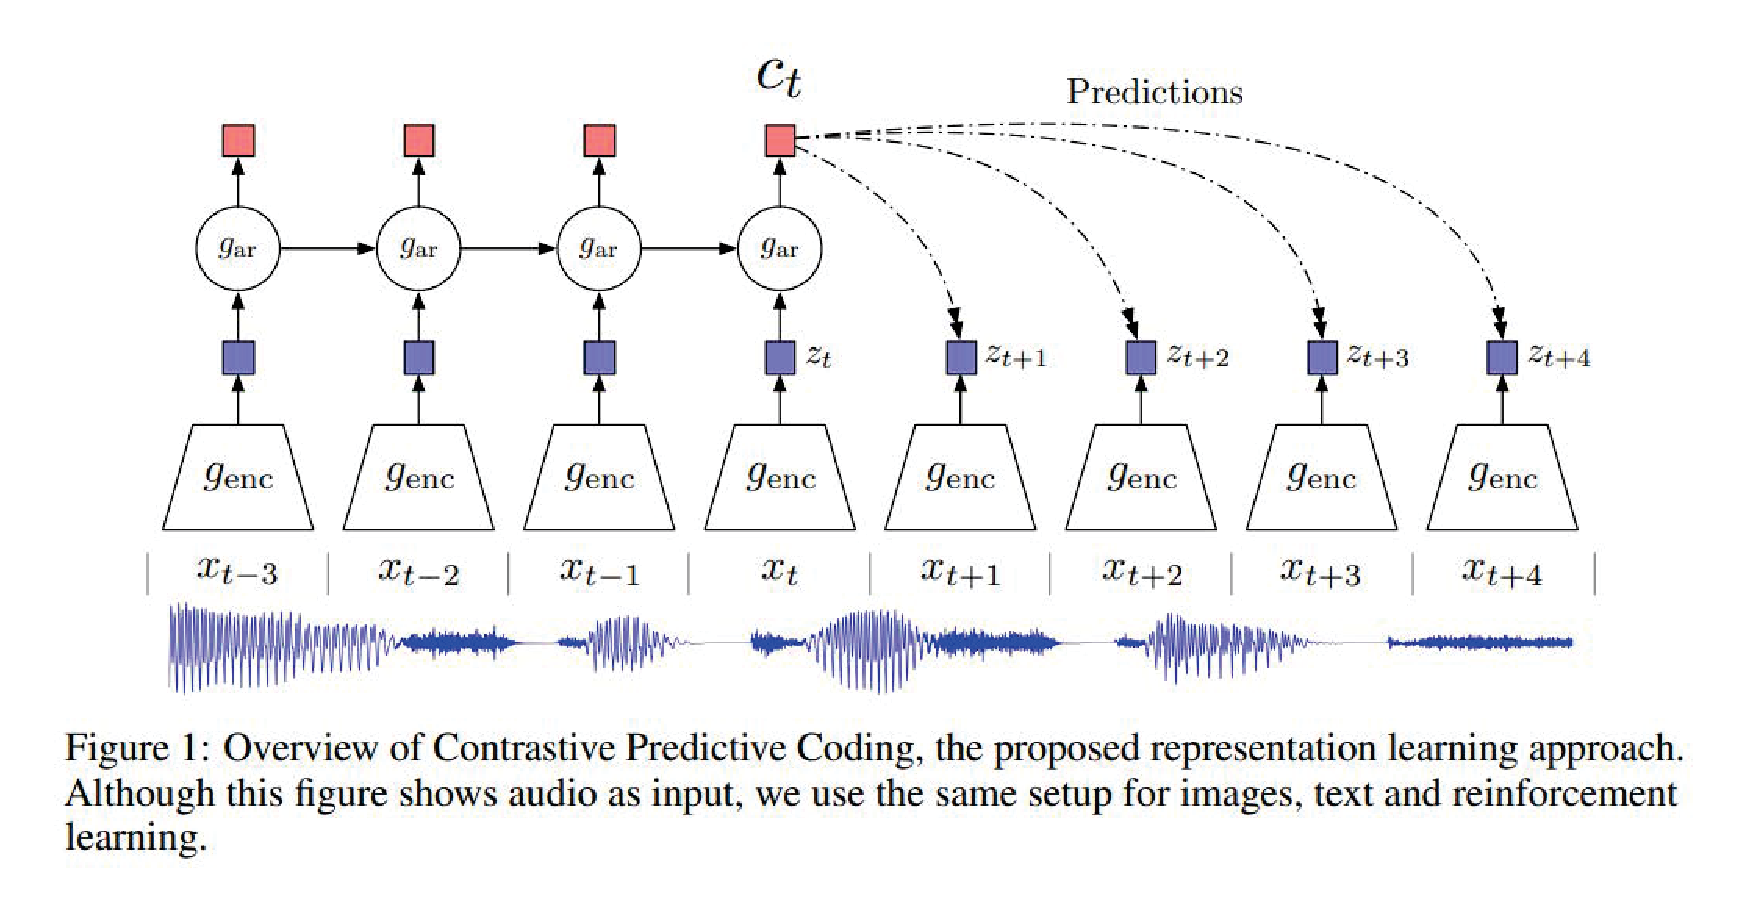
\includegraphics[width=15cm]{graphics/CPC.eps}
    \caption{Contrastive Predictive Coding}
    \label{FIG:CPC}
\end{figure}

InfoNCE是在论文 \cite{DBLP:journals/corr/abs-1807-03748} 提出的,主要用于对比预测编码(Contrastive Predictive Coding, CPC)。 
CPC核心思想是通过无监督任务来学习(编码)高维数据特征,通常采取无监督策略根据上下文预测未来或缺失的信息。
CPC示意图如上图所示。CPC的核心思想是最大化语境$c_t$与目标单词$x_{t+k}$之间的互信息,从而最大程度地减少未来$x_{t+k}$的不确定度。

\subsection{Mutual Information}

对于两个随机变量$\mathcal{X}$和$\mathcal{Y}$,如果联合概率分布为$p(x,y)$,边缘分布为$p(x)$和$p(y)$。则互信息的定义如下:
\begin{equation}
    \begin{split}
        I(\mathcal{X};\mathcal{Y}) &= \sum_{x\in\mathcal{X}} \sum_{y\in\mathcal{Y}} p(x,y)\log \frac{p(x,y)}{p(x)p(y)} \\
        &= \sum_{x\in\mathcal{X}} \sum_{y\in\mathcal{Y}} p(x,y)\log \frac{p(y)p(x|y)}{p(x)p(y)}\\
        &= \sum_{x\in\mathcal{X}} \sum_{y\in\mathcal{Y}} p(x,y)\log \frac{p(x|y)}{p(x)}\\
        &= \sum_{x\in\mathcal{X}} \sum_{y\in\mathcal{Y}} p(x,y)\log p(x|y) - \sum_{x\in\mathcal{X}} \sum_{y\in\mathcal{Y}} p(x,y)\log p(x)\\
        &= -\sum_{x\in\mathcal{X}} p(x)\log p(x) - \left[ -\sum_{x\in\mathcal{X}} \sum_{y\in\mathcal{Y}} p(x,y)\log p(x|y) \right] \\
        &= -\sum_{x\in\mathcal{X}} p(x)\log p(x) - \left[ -\sum_{x\in\mathcal{X}} \sum_{y\in\mathcal{Y}} p(x|y)p(y) \log p(x|y) \right]\\
        &= -\sum_{x\in\mathcal{X}} p(x)\log p(x) - \left[ -\sum_{x\in\mathcal{X}} p(x|y) \log p(x|y) \right]\\
        &= H(\mathcal{X}) - H(\mathcal{X}|\mathcal{Y})
    \end{split}
\end{equation}
我们可以认为,互信息$I(\mathcal{X};\mathcal{Y})$表示知道事实$\mathcal{Y}$后,原有的信息量$H(\mathcal{X})$减少了多少。
也就是说,随机变量$\mathcal{Y}$引入后,原有的随机变量$\mathcal{X}$熵(不确定度)减少的量。

\subsection{CPC}

假定有$N$个序列数据$\mathcal{X} = \{X_1, X_2, \ldots, X_N\}$。
对于其中一条序列$X = \{x_1, x_2,\ldots, x_t, x_{t+1}, \ldots, x_{t+N},\ldots\}$。
如图(\ref{FIG:CPC})所示,首先使用非线性编码器$g_{enc}$将每个观测值$x_t$映射为$z_t=g_{enc}(x_t)$。
之后再将$z_t$及之前所有时刻相关信息输入到自回归模型$g_{ar}$中,得到当前时刻上下文表示$c_t = g_{ar}(z_{\le t})$。

要构建这样的预测任务,直接的方法是建模条件生成模型$p(x_{t+k}|c_t)$,即根据当前上下文$c_t$预测$k$个时刻之后的数据$x_{t+k}$。
但是这种思路过于细节,因此作者引入\textbf{互信息}的思想,最大化当前上下文$c_t$和未来数据$x_{t+k}$之间的互信息来预测。
由于无法知道联合概率分布,因此要最大化互信息,需要最大化$\frac{p(x_{t+k}|c_{t})}{p(x_{t+k})}$。

定义$\frac{p(x_{t+k}|c_{t})}{p(x_{t+k})}$为密度比,
\begin{equation}
    f_k(x_{t+k},c_t) \propto \frac{p(x_{t+k}|c_{t})}{p(x_{t+k})}
\end{equation}
分子相当于$p_d$,相当于目标函数,分母相当于$p_n$,相当于参考分布,即噪声。
密度比$f_k(x_{t+k}, c_t)$表示上下文$c_t$的预测和未来真实值的相似程度,其正比于未来真实数据与随机采样数据的概率之比$\frac{p(x_{t+k}|c_{t})}{p(x_{t+k})}$。
在原文中,作者使用线性变换来做预测,即$W_k c_t$,$z_{t+k}$表示真实值。论文使用如下函数来逼近密度比
\begin{equation}
    f_k(x_{t+k}, c_t) = \exp(z_{t+k}^T W_k c_t)
\end{equation}

因此,根据NCE中的思路,将问题转化为二分类问题。
具体而言:
\begin{itemize}
    \item 从条件概率$p(x_{t+k}|c_t)$中采出的数据称为正样本,它是根据上下文$c_t$做出的预测数据,将正样本与上下文一起组成正样本对,类别标签设置为1.
    \item 将从$p(x_{t+k})$中取出的样本称为负样本,是与当前上下文没有必然关系的随机数据,与上下文组成负样本对,标签设置为0.
    \item 正样本也就是与$c_t$间隔步长为$k$的数据,根据NCE中的规定,正样本选取1个;因为因为NCE中证明噪声分布和数据分布越接近越好,因此负样本直接在序列中随机采样,且采的越多越好。
\end{itemize}


\subsection{InfoNCE Loss}

假定N个样本的集合$X = \{x_1, x_2, \ldots, x_N\}$包括一个正样本$p(x_{t+k}|c_t)$(从目标序列中采样得到的)和$N-1$个负样本$p(x_{t+k})$(从噪声分布中采样得到的)。
我们可以将InfoNCE Loss定义如下:
\begin{equation}
    \mathcal{L}_N = - \mathbb{E}_{X} \left[ \log \frac{f_k(x_{t+k}, c_t)}{\sum_{x_j\in X} f_k(x_j, c_t)} \right]
\end{equation}
在这个损失函数中
\begin{itemize}
    \item 如果模型性能好:那么分子会比较大,且分子中除了$j=i$这一项,其他项近乎与0。那么整个Loss会趋近于-1.
    \item 如果模型性能很差,那么Loss会趋向于$\frac{-1}{N}$。
\end{itemize}
因此,只需要最小化$\mathcal{L}$就是在优化神经网络,也就是希望神经网络将正例与负例分开。


假定$x_{t+k}$为正样本且$i=t+k$,损失函数的最佳情况如下式所示:
\begin{equation}
    \begin{split}
        p(d=i|X,c_t) &= \frac{p(d=i, X, c_t)}{p(X,c_t)} \\
        &= \frac{ p(x_i|c_t) \prod_{l \neq i} p(x_l) }{\sum_{j=1}^N p(x_j|c_t) \prod_{l \neq j} p(x_l) } \\
        &= \frac{\frac{p(x_i|c_t)}{p(x_i)}}{\sum_{j=1}^N \frac{p(x_j|c_t)}{p(x_j)}}
    \end{split}
    \label{EQ:ExampleEQU}
\end{equation}
这里要解释几个点:
\begin{itemize}
    \item 密度比$f_k(x_{t+k}, c_t)$表示预测值和真实值的相似程度。由上式最后一步,我们可以看到它确实正比于$\frac{p(x_{t+k}|c_{t})}{p(x_{t+k})}$。系数为$\frac{1}{\sum_{j=1}^N \frac{p(x_j|c_t)}{p(x_j)}}$
    \item 为什么要概率连乘呢?本质上每个$p(\cdot)$对应着一个函数,我们只是通过采集的样本,输入函数计算输出,再根据损失函数结果来更新参数。
\end{itemize}


\subsection{MI与InfoNCE之间的关系}


\begin{equation}
    \begin{split}
        \mathcal{L}_N^{opt} &= - \mathbb{E}_{X} \log [\frac{\frac{p(x_{t+k}|c_t)}{p(x_{t+k})}}{\frac{p(x_{t+k}|c_t)}{p(x_{t+k})} + \sum_{x_j \in X_{neg}} \frac{p(x_j|c_t)}{p(x_j)} }] \\
        &= \mathbb{E}_{X} \log [1+ \frac{p(x_{t+k})}{p(x_{t+k}|c_t)} \sum_{x_j \in X_{neg}} \frac{p(x_j|c_t)}{p(x_j)}] \\
        &\approx \mathbb{E}_X \log [1+ \frac{p(x_{t+k})}{p(x_{t+k}|c_t)} (N-1) \mathbb{E}_{x_j}\frac{p(x_j|c_t)}{p(x_j)}] \\
        &=  \mathbb{E}_X \log [1+ \frac{p(x_{t+k})}{p(x_{t+k}|c_t)} (N-1)] // \textbf{因为负例随机取,与上下文无关}\\
        &\ge \mathbb{E}_X \log [\frac{p(x_{t+k})}{p(x_{t+k}|c_t)} N]\\
        &= -I(x_{t+k},c_t)+ \log(N)
    \end{split}
\end{equation}

由上式可以看出,优化InfoNCE也就是最大化$\mathcal{L}^{opt}$和$c_t$之间互信息的下限。并且N越大,约等于越准确。

\section{附录:NEG/NCE/GAN/SSL之间的关系}

能量启发模型(EIM):从负采样到自监督学习(NEG-NCE(InfoNCE)-GAN-SSL 家族):\url{https://zhuanlan.zhihu.com/p/413681189}


总体结论如下:
\begin{itemize}
    \item 负采样(NEG)是对噪声对比估计(NCE)的近似
    \item 噪声对比估计(NCE)是对极大似然估计(MLE)的近似
    \item 噪声对比估计(NCE)是生成器固定的生成对抗网络(GAN)
    \item InfoNCE是多分类版本的噪声对比估计(NCE)
    \item InfoNCE及其变体是自监督学习(SSL)常用的损失函数
    \item InfoNCE实质上是在做自归一重要性采样(SNIS)
    \item 以上模型都是在回避对配分函数的直接计算
\end{itemize}

里面有一些问题:

\paragraph{【NEG部分】为什么分类模型为:}

\begin{equation}
    \begin{cases}
        p(D=1|w_t, w_{t+j}) = \sigma(u^T_{w_{t+j}} v_{w_t})\\
        p(D=0|w_t, w_k) = 1-\sigma(u^T_{w_k} v_{w_t})
    \end{cases}
\end{equation}
答:因为这只是个二分类函数,Logistic Regression是常用的而已。

\paragraph{【NEG v.s. NCE】为什么NEG只可以生成词嵌入,而不能生成语言模型?}

答:因为NEG只关注分类,而语言模型的核心是$p(w|c)$,是条件概率,处于$\left[0,1\right]$。而NEG得到的表示未经过归一化,不是概率。

\paragraph{【NCE v.s. IS】配分函数中的约等于号是为什么?}

\begin{equation}
    \begin{split}
        p(D=1|w_t, w_{t+j}) &= \sigma(\Delta S_{\theta^0}(w,v))\\
        &= \frac{1}{1+\exp (- \Delta S_{\theta^0} (w,v)))} \\
        &= \frac{\exp (\Delta S_{\theta^0} (w,v))}{\exp (\Delta S_{\theta^0} (w,v)) + 1} \\
        &= \frac{\exp(S_{\theta^0}(w,v) - \log K \cdot p_n(w))}{\exp(S_{\theta^0}(w,v) - \log K \cdot p_n(w)) + 1} \\
        &= \frac{ \frac{\exp(S_{\theta^0}(w,v))}{\exp (\log K \cdot p_n(w) )} }{\frac{\exp(S_{\theta^0}(w,v))}{\exp (\log K \cdot p_n(w) )}+1} \\
        &= \frac{\exp(S_{\theta^0}(w,v))}{\exp(S_{\theta^0}(w,v))+K\cdot p_n(w)}\\
    \end{split}
\end{equation}

而前文提到,使用$p_{data}$去近似$p_\theta$。而如公式(\ref{EQ:ExpAndZ})和(\ref{EQ:Theta0})所示
\begin{equation}
    p_\theta(w|c) = p_{\theta^0}(w|c)\exp (z_c) = \exp(s_{\theta^0}(w|c))\exp (z_c) = u_{\theta^0}(w,c)
\end{equation}
因此,相当于约掉了$\exp(z_c)$


\bibliographystyle{apalike}
\bibliography{ref}

\end{document}